\chapter{Data and Methodology}
\label{ch:ch3}

This chapter describes the data source, the derivation of the analytical sample, the variable set, the preprocessing decisions, the three complementary analytical approaches employed for the segmentation of the elderly population, and the validation strategy. The pipeline is applied identically to Italy and Sweden to ensure cross-country comparability, with the only intentional country-specific deviation documented in Section~\ref{sec:ch3-variables}.

\section{Data source}
\label{sec:ch3-data}

The Survey of Health, Ageing and Retirement in Europe (SHARE) provides the empirical foundation of this thesis. Launched in 2004 and coordinated by the Max Planck Institute for Social Law and Social Policy, SHARE fields a harmonised battery of health, economic, cognitive, and social-network instruments across twenty-seven European countries and a complementary Israeli sample (Börsch-Supan et al., 2013). The ninth wave (SHARE W9), fielded between 2021 and 2022 and used throughout this thesis, includes 5{,}601 Italian and 3{,}405 Swedish respondents (SHARE Release 9.0.0, 2024). The harmonised questionnaire, cross-national coverage, and post-pandemic timing of W9 make it particularly suited to the comparative welfare-regime question addressed here.

Three methodological advantages justify the choice of SHARE W9. First, the strictly harmonised questionnaire permits direct cross-national comparisons on identical indicator batteries, a necessary condition for welfare-regime comparative designs (Esping-Andersen, 1990; Ferrera, 1996). Second, the integration of health, financial, digital, cognitive and subjective measures within a single instrument enables the multidimensional segmentation that constitutes the core analytical strategy of this thesis. Third, the W9 fieldwork captures the elderly population immediately after the most acute phase of the COVID-19 pandemic, a period in which digital integration and social isolation acquired unprecedented policy salience (Seifert et al., 2021).

The analysis focuses on two country sub-samples: Italy (country code 16 in SHARE) and Sweden (country code 13). These two cases exemplify polar welfare-regime types --- the familistic, Mediterranean model and the universalist, Social-Democratic model respectively (Esping-Andersen, 1990; Ferrera, 1996) --- and their comparison is empirically rich yet analytically tractable. The contrast also maps directly onto the thesis's substantive interest in how welfare architecture conditions the multidimensional experience of ageing, while controlling for the shared institutional context of the European Union and the common measurement apparatus of SHARE.

\section{Analytical sample derivation}
\label{sec:ch3-sample}

Figure~\ref{fig:ch3-sample-flow} documents the derivation of the analytical samples from the raw SHARE W9 files. Three successive restrictions were applied to each country.

\begin{figure}[ht]
  \centering
  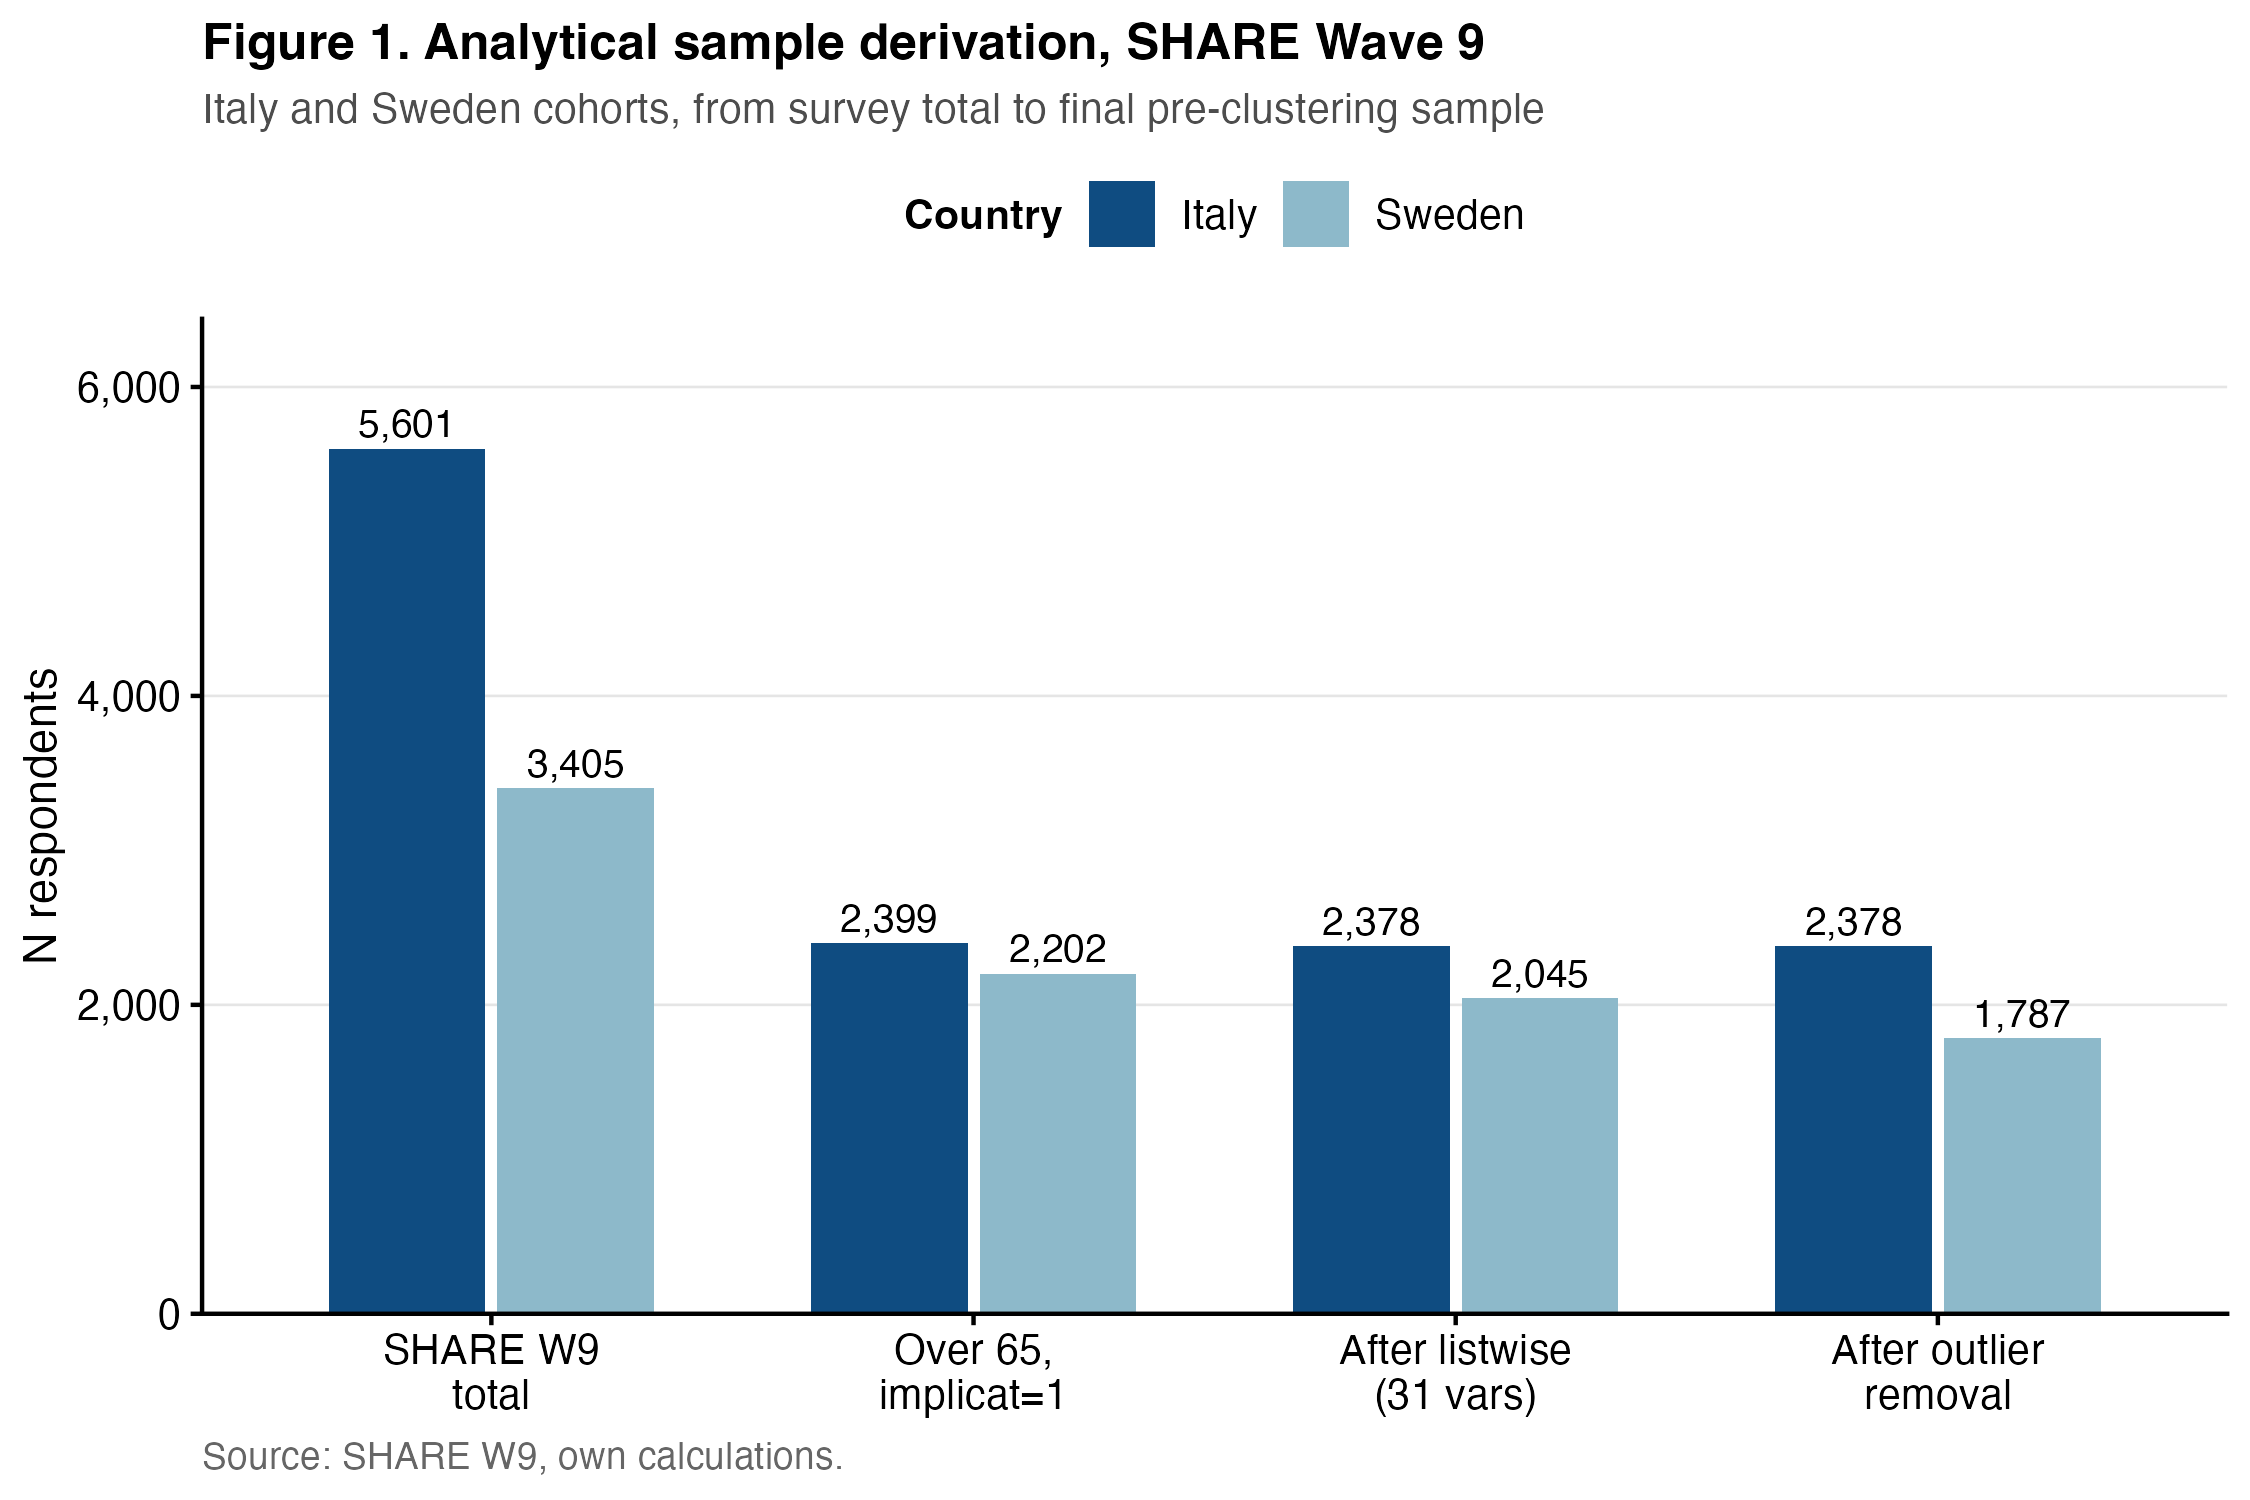
\includegraphics[width=0.85\linewidth]{figures/03_data_methods/fig_01_sample_flow.png}
  \caption{Analytical sample derivation, SHARE Wave 9. Italy and Sweden cohorts, from survey total to final pre-clustering sample. Source: SHARE W9, own calculations.}
  \label{fig:ch3-sample-flow}
\end{figure}

First, the analysis was limited to non-institutionalised respondents aged sixty-five years or older at the time of interview, retaining only the first implicate produced by SHARE's multiple-imputation procedure (\emph{implicat~==~1}). This restriction reduces the working samples to 2{,}399 (Italy) and 2{,}202 (Sweden) observations, consistent with the population of interest for research on ageing.

Second, complete-case listwise deletion was applied across the thirty-one analytical variables described in Section~\ref{sec:ch3-variables}. Listwise deletion, rather than multiple imputation, was chosen because the clustering and factor-analytic procedures at the centre of the analytical strategy require fully observed cases, and because the amount of missingness is modest and approximately missing-at-random on the selected items (Little \& Rubin, 2019). After this step the Italian sample stands at 2{,}378 respondents and the Swedish sample at 2{,}045.

Third, multivariate outliers were identified using the Mahalanobis distance against the correlation structure of the thirty-one standardised variables. A conservative $\chi^{2}$ cut-off at $p = 0.001$ (31 degrees of freedom) was adopted to avoid overly aggressive trimming. No Italian respondent exceeds the cut-off; 258 Swedish cases are flagged and removed. The final analytical samples are therefore $n = 2{,}378$ (Italy) and $n = 1{,}787$ (Sweden).

It should be noted that these final sample sizes differ from those reported in earlier iterations of the project design. This divergence reflects the adoption of a uniform, code-authoritative preprocessing pipeline that applies the same Mahalanobis threshold to both countries and does not rely on any previously computed cleaning artefacts. All empirical results presented in the remainder of the thesis derive from the samples described above.

\section{Variables}
\label{sec:ch3-variables}

The thirty-one analytical variables span five conceptual dimensions --- health, economic resources, digital and social engagement, cognitive function, and subjective well-being --- summarised in Table~\ref{tab:ch3-variables}. The selection replicates, within SHARE W9, the multidimensional structure of successful ageing proposed by Rowe and Kahn (1997), while incorporating the post-pandemic emphasis on digital inclusion that motivates much current research on ageing societies (Friemel, 2016; König et al., 2018).

\begin{table}[ht]
  \centering
  \caption{Analytical variables by conceptual dimension.}
  \label{tab:ch3-variables}
  \small
  \begin{tabular}{@{}lp{9.5cm}@{}}
    \toprule
    \textbf{Dimension} & \textbf{Variables}\\
    \midrule
    Health (8)               & \emph{sphus}, \emph{chronic}, \emph{adl}, \emph{iadl}, \emph{mobility}, \emph{eurod}, \emph{bmi}, \emph{phinact}\\
    Economic resources (5)   & \emph{log\_thinc}, \emph{log\_hnetw}, \emph{ypen1}, \emph{home\_own}, \emph{fdistress}\\
    Digital / social (10)    & \emph{internet}, \emph{ac035d1}, \emph{ac035d5}, \emph{ac035d8}, \emph{sp002\_}, \emph{sp008\_}, \emph{sn\_size\_w9}, \emph{social\_integration}, \emph{ac035d4}, \emph{ac035d7}\\
    Cognitive (3)            & \emph{fluency}, \emph{memory}, \emph{orienti}\\
    Subjective well-being (5)& \emph{loneliness}, \emph{casp}, \emph{hope\_future}, \emph{interest}, \emph{expect\_alive}\\
    \bottomrule
  \end{tabular}
  \par\smallskip
  \footnotesize \emph{Note.} Eleven variables are binary (\emph{phinact}, \emph{home\_own}, \emph{internet}, \emph{ac035d1}, \emph{ac035d5}, \emph{ac035d8}, \emph{sp002\_}, \emph{sp008\_}, \emph{ac035d4}, \emph{ac035d7}, \emph{hope\_future}); the remaining twenty are continuous or quasi-continuous. Short human-readable labels and measurement scales are given in Figures~4, 5, 34, 50, 51, 66 and~67; the full mapping is stored in the helper module \texttt{v9/var\_labels.R}.
\end{table}

Eleven of the thirty-one variables are binary (coded 0/1); twenty are continuous or quasi-continuous. Three SHARE items that might in principle have entered the analytical battery were excluded on grounds of cross-country comparability. The item \emph{pcskill\_r} (computer skills self-assessment) is administered only to respondents who report regular personal-computer use, yielding 48 per cent missing values in Sweden; the items \emph{wllft} and \emph{wllst} (immediate and delayed word recall) cover 22 and 25 per cent of the Swedish sample respectively, because they are administered only to a random sub-sample of participants. Retaining these items would have forced a much smaller common support, distorting the comparative exercise.

Two digital-engagement items require particular comment. In Italy, \emph{ac035d4} (participation in educational training) and \emph{ac035d7} (involvement in political organisations) have zero variance: no Italian respondent in the analytical sample reports either activity. This pattern appears to reflect an artefact of the Italian fieldwork rather than a substantive finding about participation, but it requires the two variables to be excluded from the Italian PCA and factor-analysis computations. In Sweden the same items exhibit low but non-zero variance (four to six per cent positive responses) and are therefore retained. The common analytical battery comprises twenty-nine active variables in Italy and thirty-one in Sweden; cross-country comparisons at the profile level rely on indicators that are active in both countries.

\section{Preprocessing}
\label{sec:ch3-preprocessing}

Two successive transformations were applied to the twenty non-binary variables prior to analysis, following the workflow established in the Bocconi course 20570 \emph{Data Analytics and Visualization} (Piccareta \& Trentini, 2025). First, each non-binary variable was rank-transformed using average-rank tie-breaking. Rank transformation uniformises marginal distributions and mitigates the influence of extreme values on the distance-based procedures that follow, at the cost of discarding information about absolute magnitudes. Second, every analytical variable --- binary and non-binary alike --- was standardised to zero mean and unit variance (z-score standardisation), so that no dimension dominates cluster formation or factor extraction by virtue of its original scale.

Binary variables were not rank-transformed, since the rank of a 0/1 variable collapses into a trivial two-valued distribution. They were nevertheless z-standardised jointly with the continuous variables, yielding a single homogeneous standardised matrix of thirty-one columns for Sweden and twenty-nine columns for Italy. This homogeneous standardised matrix is the direct input to the K-means, PCA, and factor-analysis procedures described below. For the Latent Class Analysis of Section~\ref{sec:ch3-lca}, the continuous variables are further discretised into tertiles, as detailed there.

\section{Analytical framework}
\label{sec:ch3-framework}

The empirical strategy of this thesis employs three complementary methods to produce and validate the multidimensional profiles of elderly Italians and Swedes. Each method rests on a different theoretical premise and draws on a different statistical tradition, and their triangulation serves to evaluate whether a given profile reflects a robust population type or a method-specific artefact (Magidson \& Vermunt, 2002).

\subsection{Dimension-wise Principal Component Analysis}
\label{sec:ch3-pca}

Principal Component Analysis (PCA) was applied separately to each of the five conceptual dimensions. This dimension-wise decomposition serves three purposes: it summarises the correlational structure of the three to ten indicators within each dimension into a smaller set of orthogonal components; it provides diagnostics for the presence of a natural latent structure within each domain; and it anchors the downstream outlier analysis that flagged Swedish extreme respondents.

Components were retained on the basis of Kaiser's criterion (eigenvalue greater than one), with one documented exception. For the digital/social block, four components were retained in both countries even though the fourth component has an eigenvalue just below unity (0.96 in Italy, 0.98 in Sweden). Two considerations motivated this departure. First, when Kaiser's threshold lies so near one, the criterion provides only weak guidance. Second, the fourth component carries meaningful substantive content --- it captures a latent axis of civic and political engagement independent of generic digital use --- and the ensuing outlier diagnostics depend on it to flag extreme respondents. Retaining four components therefore maximises comparability with the reference design and ensures that the cross-country profile structures remain commensurable.

\subsection{Factor analysis}
\label{sec:ch3-fa}

A second lens on the variable space is provided by exploratory factor analysis, fitted with principal-axis extraction, varimax rotation, and six factors per country. Factor analysis differs from PCA in two respects: it isolates the shared-variance component of each indicator, discarding uniquenesses, and it rotates the latent space to approximate simple structure (each indicator loading primarily on one factor). The course treats factor analysis as the preferred tool for substantive interpretation of latent constructs (Piccareta \& Trentini, 2025), while reserving PCA for dimensionality reduction.

The six-factor solution is justified \emph{ex ante} by theoretical expectations --- five substantive dimensions plus a mood-versus-cognition distinction within the subjective block --- and \emph{ex post} by empirical diagnostics. The Kaiser--Meyer--Olkin measure of sampling adequacy equals 0.832 in Italy and 0.808 in Sweden, both above the meritorious threshold (Kaiser \& Rice, 1974). Bartlett's test of sphericity is rejected at any conventional level in both countries ($\chi^{2} = 18{,}755$, $df = 406$ for Italy; $\chi^{2} = 9{,}067$, $df = 465$ for Sweden; both $p < 10^{-300}$). Parallel analysis with one hundred random datasets suggests ten factors in Italy and nine in Sweden; Kaiser's criterion on the full correlation matrix indicates nine and ten respectively. The six-factor solution is therefore conservative and is retained on interpretive grounds and for cross-country comparability, with the BIC-minimal larger solutions reported as sensitivity analyses in Chapter~6.

One diagnostic deserves explicit mention: in Sweden, \emph{social\_integration} exhibits a Heywood case with an estimated loading of 1.11 on its dominant factor, yielding a communality of 1.38 once small secondary loadings are added in quadrature. This pattern reflects the near-perfect determination of the social-integration index by its dominant factor; it is flagged rather than treated. Chapter~6 discusses its implications for the stability of the Swedish solution and evaluates alternative parameterisations.

\subsection{K-means clustering}
\label{sec:ch3-kmeans}

The core segmentation device of this thesis is K-means clustering, applied to the thirty-one (respectively twenty-nine) standardised variables rather than to any factor- or component-derived score. This choice follows the methodological guidance of course 20570 (Piccareta \& Trentini, 2025) and ensures that profile means can be interpreted directly in the metric of the original indicators. Clustering on factor scores is sometimes preferred in the literature on latent-variable segmentation (Magidson \& Vermunt, 2002), but it complicates the interpretation of profile characteristics and, as shown in Chapter~6, may produce unstable assignments when the factor solution itself contains Heywood cases.

For each country, K-means was initialised with one hundred random restarts, a maximum of five hundred iterations per restart, and a fixed random seed (42) for reproducibility. The number of clusters was fixed at six for both countries at the model-fitting stage, consistent with the reference design. In Italy, the six-cluster solution was subsequently refined by removing any micro-cluster smaller than five per cent of the sample and characterised by extreme digital-component scores; at $n = 2{,}378$ no such micro-cluster emerged, and the analysis was refitted directly with $k = 5$ on the full sample. In Sweden the six-cluster solution was retained without further removal, since no micro-cluster emerged --- a pattern that is consistent with the reference design's observation that the Italian micro-cluster has no Swedish analogue.

K-means was preferred over hierarchical alternatives on empirical grounds. The within-cluster quality indexes computed across $k = 2,\ldots,12$ show that K-means attains uniformly higher within-cluster $R^{2}$ and silhouette than Ward, complete, and average linkage in both countries; Ward only rivals K-means on the Dunn index, which penalises cluster elongation differently. This comparison is summarised in Figures~22--23 (K-means diagnostics by country) and in the multi-algorithm overlay of Figures~64--65, which presents all six indexes ($R^{2}$, Pseudo-F, silhouette, Davies-Bouldin proxy, Dunn and Pearson--gamma) for the four algorithms on a common scale. Figures~66--67 further document, variable by variable, how the within-cluster $R^{2}$ saturates with $k$ for each algorithm, highlighting a small group of indicators (e.g.\ body mass index, received help) that carry no clustering signal under any method and a larger group whose separation stabilises precisely in the $k = 5,\ldots,6$ range.

The choice of $k = 5$ for Italy and $k = 6$ for Sweden rests on three converging criteria. First, the silhouette and $R^{2}$ curves of Figures~22--23 flatten beyond these values, indicating diminishing returns from further partitioning. Second, the semi-partial $R^{2}$ and Pseudo-$T^{2}$ (Duda--Hart) diagnostics reported in the appendix (Figures~72--73) display the sharpest merge-cost jumps when $k$ crosses the chosen cut-off, consistent with a natural boundary in the dendrogram. Third, the five- and six-cluster solutions produce substantively interpretable profiles that map onto the welfare-regime hypotheses of Chapter~5; solutions with $k > 6$ split the Connected and Social profiles into thematically redundant fragments, while $k < 5$ collapses the Fragile Resigned / Fragile Depressed contrast that is the analytical payoff of the subjective-wellbeing block.

\subsection{Latent Class Analysis}
\label{sec:ch3-lca}

A third, probabilistic lens on the same population is provided by Latent Class Analysis (LCA), fitted using the R package \emph{poLCA} (Linzer \& Lewis, 2011). LCA models the joint distribution of categorical indicators as a mixture of latent-class-specific multinomial distributions, yielding a fully probabilistic assignment of respondents to classes. Whereas K-means imposes hard, distance-based partitions, LCA produces posterior probabilities over all latent classes for every individual and thus supports a more explicit assessment of classification uncertainty (Collins \& Lanza, 2010).

\emph{poLCA} requires categorical indicators, so the twenty non-binary variables were discretised into tertiles (1 = low, 2 = mid, 3 = high) prior to fitting. Five variables whose distributions are heavily zero-inflated --- \emph{adl}, \emph{iadl}, \emph{memory}, \emph{orienti} and \emph{interest} --- admit only two or two-plus-one effective categories; for these a mode-based split was adopted (one category for the modal value, one or two for the remainder). For each country, LCA was estimated for $k = 2$ through $k = 8$ with five random restarts and up to one thousand EM iterations per fit. Normalised entropy (computed from the posterior matrix) and the Bayesian Information Criterion are reported for all fits. Chapter~6 uses these criteria, alongside the cluster-level convergence between K-means and LCA assignments, to evaluate the robustness of the segmentation.

\section{Validation strategy}
\label{sec:ch3-validation}

Three complementary validation strategies are used throughout the thesis.

First, external validation exploits a variable that did not enter the clustering. Life satisfaction --- measured on the SHARE zero-to-ten scale (\emph{ac012\_}) and absent from the analytical battery --- is regressed on the profile factor through a one-way analysis of variance (ANOVA) in each country. A strong between-group effect indicates that the profiles capture real variation in aspects of well-being that were not used in their construction. Welch's $t$-test and Tukey's HSD are used for post-hoc pairwise comparisons and adjust for unequal variances and multiplicity.

Second, internal consistency is assessed by comparing K-means and LCA assignments on the same individuals. A cluster-specific convergence rate is computed as the share of members of a given K-means profile that are also assigned to the modal LCA class. High convergence indicates a robust latent type, while low convergence flags a profile that is geometrically well-defined but probabilistically ambiguous.

Third, cross-country comparability is evaluated through four matched profile pairs constructed to correspond semantically across Italy and Sweden, as detailed in Table~\ref{tab:ch3-matched-pairs}. Welch's $t$-tests compare the Italian and Swedish members of each pair on the core well-being and connectedness variables, and chi-squared tests perform the analogous comparison on binary indicators. Profiles that have no cross-country analogue are reported separately as welfare-regime-specific types and listed in the bottom row of Table~\ref{tab:ch3-matched-pairs}.

\begin{table}[ht]
  \centering
  \caption{Cross-country matched-pair mapping between Italian and Swedish profiles.}
  \label{tab:ch3-matched-pairs}
  \small
  \begin{tabular}{@{}lll@{}}
    \toprule
    \textbf{Matched pair} & \textbf{Italian profile} & \textbf{Swedish profile}\\
    \midrule
    Fragile            & \emph{Fragile Resigned}   & \emph{Fragile}\\
    Declining          & \emph{Fragile Depressed}  & \emph{Social Decline}\\
    Socially-oriented  & \emph{Traditional Social} & \emph{Moderate}\\
    Connected          & \emph{Connected Active}   & \emph{Connected Wealthy}\\
    \midrule
    Unmatched          & \emph{Moderate Isolated}  & \emph{Asset Rich}, \emph{Wealthy Digital}\\
    \bottomrule
  \end{tabular}
  \par\smallskip
  \footnotesize \emph{Note.} Profiles in the first four rows are compared on well-being and connectedness variables via Welch's $t$-tests and chi-squared tests. Profiles in the bottom row have no cross-country analogue and are reported as welfare-regime-specific types in Chapter~5.
\end{table}

\section{Software and reproducibility}
\label{sec:ch3-software}

All analyses were conducted in R 4.5 (R Core Team, 2024) with the following principal packages: \emph{psych} 2.3 (factor analysis and KMO/Bartlett diagnostics), \emph{cluster} 2.1 (silhouette computation), \emph{poLCA} 1.6 (latent class analysis), \emph{haven} 2.5 (reading SHARE Stata files), and the \emph{tidyverse} suite (data manipulation and visualisation). The analytical pipeline is organised into twenty numbered R scripts --- from raw SHARE file ingestion to final figure generation --- together with two shared helper modules: a central variable-label dictionary (\texttt{v9/var\_labels.R}) and a chapter-routing utility (\texttt{v9/fig\_paths.R}) that deposits each figure under the appropriate chapter subfolder. All twenty-two files are available in the online appendix. Each script uses a fixed random seed (42) wherever stochasticity is involved; the total execution time from raw files to final figures is approximately forty minutes on a standard laptop, with the cluster-diagnostic scripts (hierarchical linkages over $k = 2,\ldots,12$) accounting for the bulk of the runtime.

Raw SHARE data are used under the conditions of Release 9.0.0, which require an end-user licence and prohibit disclosure of individual-level data. All aggregate results and figures presented in this thesis comply with the SHARE publication guidelines; no individual respondent is identifiable from the results reported.
